\documentclass[10pt,adobefonts,fancyhdr,hyperref,UTF8]{ctexbook}

\usepackage{multirow}
% for \soul 删除线
\usepackage{ulem}
% 表头斜线
\usepackage{diagbox}

\makeatletter
\usepackage[centering,paperwidth=180mm,paperheight=230mm,%
body={390pt,530pt},marginparsep=10pt,marginpar=50pt]{geometry}
\usepackage{color}
\usepackage{enumitem}
\usepackage{fancyvrb}
\usepackage[bottom,perpage,symbol*]{footmisc}
\usepackage{graphicx}
\usepackage[hidelinks]{hyperref}
\usepackage{makeidx}
\usepackage[toc]{multitoc}
\usepackage{pifont}
\usepackage{underscore}
\usepackage{amsmath}

\DefineFNsymbols*{chinese}{{\ding{172}}{\ding{173}}{\ding{174}}{\ding{175}}%
{\ding{176}}{\ding{177}}{\ding{178}}{\ding{179}}{\ding{180}}{\ding{181}}}
\setfnsymbol{chinese}

\hypersetup{bookmarksnumbered=true,bookmarksdepth=2}

\CTEXsetup[number={\thechapter}]{chapter}
\CTEXsetup[format+={\raggedleft}]{chapter}
\CTEXsetup[beforeskip={10pt}]{chapter}
\CTEXsetup[afterskip={30pt}]{chapter}
\def\CTEX@chapter@aftername{\par} % \CTEXsetup[aftername={\par}]{chapter}
\CTEXsetup[format+={\raggedright}]{section}
\CTEXsetup[beforeskip={-3.0ex plus -1ex minus -.2ex}]{section}
\CTEXsetup[afterskip={2.3ex plus .2ex minus 0.2ex}]{section}

\renewcommand \thefigure{\thechapter-\arabic{figure}}
\renewcommand \thetable{\thechapter-\arabic{table}}

\newcommand\figcaption[1]{\def\@captype{figure}\caption{#1}}
\newcommand\tabcaption[1]{\def\@captype{table}\caption{#1}}

\long\def\@caption#1[#2]#3{%
  \addcontentsline{\csname ext@#1\endcsname}{#1}%
    {\protect\numberline{\csname fnum@#1\endcsname}{ \ignorespaces #2}}% change "the" to "fnum@"
    \normalsize
    \@makecaption{\csname fnum@#1\endcsname}{\ignorespaces #3}}

\long\def\@makecaption#1#2{%
  \vskip\abovecaptionskip
  \sbox\@tempboxa{#1\quad#2}%
  \ifdim \wd\@tempboxa >\hsize
    #1\quad#2\par
  \else
    \global \@minipagefalse
    \hb@xt@\hsize{\hfil\box\@tempboxa\hfil}%
  \fi
  \vskip\belowcaptionskip}

\setlength\abovecaptionskip{0pt}
  
\setmainfont{Times New Roman}
%\setmainfont{Linux Libertine}
%\setmainfont{TeX Gyre Pagella}
\newfontfamily\urlfont{PT Sans Narrow}
%\setmonofont[AutoFakeBold=1.6,AutoFakeSlant=0.17,Mapping=tex-text-tt]{Inconsolata}
\setCJKfamilyfont{zhyou}{YouYuan}

\newcommand{\fn}[1]{\texttt{#1}}
\newcommand{\sfn}[1]{\texttt{\small #1}}
\newcommand{\kw}[1]{\textsf{#1}}
\newcommand{\myurl}[1]{{\urlfont #1}}
\newcommand{\mpar}[1]{\marginpar[\hfill\kaishu #1]{\kaishu #1}}
\newcommand{\mn}[1]{\texttt{\bs #1}}
\renewcommand{\today}{\the\year-\the\month-\the\day}
\newcommand\bs{\textbackslash}
\newcommand{\code}[1]{\small{\fontspec{Latin Modern Mono} #1}}

\newcommand\begindot{\begin{itemize}
[itemsep=2pt plus 2pt minus 2pt,%
topsep=3pt plus 2pt minus 2pt,%
parsep=0pt plus 2pt minus 2pt]}
\newcommand\myenddot{\end{itemize}}

\newcommand\beginnum{\begin{enumerate}
[itemsep=2pt plus 2pt minus 2pt,%
topsep=3pt plus 2pt minus 2pt,%
parsep=0pt plus 2pt minus 2pt]}
\newcommand\myendnum{\end{enumerate}}

\DefineVerbatimEnvironment%
  {Code}{Verbatim}
  {fontsize=\small,baselinestretch=0.9,xleftmargin=3mm}

\raggedbottom
%\setlength{\parskip}{1ex plus .5ex minus .5ex}

\def\FV@SetLineWidth{%
  \if@FV@ResetMargins\else
    \advance\leftmargin\@totalleftmargin
  \fi
  \advance\leftmargin\FV@XLeftMargin\relax
  \advance\rightmargin\FV@XRightMargin\relax
  \linewidth\hsize
  %\advance\linewidth-\leftmargin
  %\advance\linewidth-\rightmargin
  \hfuzz\FancyVerbHFuzz\relax}


\def\FV@SingleFrameLine#1{%
%% DG/SR modification end
  \hbox to\z@{%
    %\kern\leftmargin
%% DG/SR modification begin - Jun. 22, 1998
    \ifnum#1=\z@
      \let\FV@Label\FV@LabelBegin
    \else
      \let\FV@Label\FV@LabelEnd
    \fi
    \ifx\FV@Label\relax
%% DG/SR modification end
      \FancyVerbRuleColor{\vrule \@width\linewidth \@height\FV@FrameRule}%
%% DG/SR modification begin - Jun. 22, 1998
    \else
      \ifnum#1=\z@
        \setbox\z@\hbox{\strut\enspace\urlfont\FV@LabelBegin\strut}%
      \else
        \setbox\z@\hbox{\strut\enspace\urlfont\FV@LabelEnd\strut}%
      \fi
      \@tempdimb=\dp\z@
      \advance\@tempdimb -.5\ht\z@
      \@tempdimc=\linewidth
      \advance\@tempdimc -\wd\z@
      %\divide\@tempdimc\tw@
      \ifnum#1=\z@              % Top line
        \ifx\FV@LabelPositionTopLine\relax
          \FancyVerbRuleColor{\vrule \@width\linewidth \@height\FV@FrameRule}%
        \else
          \FV@FrameLineWithLabel
        \fi
      \else                     % Bottom line
        \ifx\FV@LabelPositionBottomLine\relax
          \FancyVerbRuleColor{\vrule \@width\linewidth \@height\FV@FrameRule}%
        \else
          \FV@FrameLineWithLabel
        \fi
      \fi
    \fi
%% DG/SR modification end
    \hss}}


%% DG/SR modification begin - May. 19, 1998
\def\FV@FrameLineWithLabel{%
  \ht\z@\@tempdimb\dp\z@\@tempdimb%
  \FancyVerbRuleColor{%
    \raise 0.5ex\hbox{\vrule \@width\@tempdimc \@height\FV@FrameRule}%
    \raise\@tempdimb\box\z@}}
%% DG/SR modification end


\def\FV@EndListFrame@Lines{%
  \begingroup
    %\vskip 0.5ex
    \baselineskip\z@skip
    \kern\FV@FrameSep\relax
%% DG/SR modification begin - May. 19, 1998
%%    \FV@SingleFrameLine
    \FV@SingleFrameLine{\@ne}%
%% DG/SR modification end
  \endgroup}

\newskip\mytopsep
\setlength{\mytopsep}{4pt plus 2pt minus 3pt}

\def\FV@ListVSpace{%
  \@topsepadd\mytopsep
  \if@noparlist\advance\@topsepadd\partopsep\fi
  \if@inlabel
    \vskip\parskip
  \else
    \if@nobreak
      \vskip\parskip
      \clubpenalty\@M
    \else
      \addpenalty\@beginparpenalty
      \@topsep\@topsepadd
      \advance\@topsep\parskip
      \addvspace\@topsep
    \fi
  \fi
  %\showthe \@topsepadd
  %\showthe \topsep
  %\showthe \partopsep
  %\showthe \parskip
  \global\@nobreakfalse
  \global\@inlabelfalse
  \global\@minipagefalse
  \global\@newlistfalse}

\def\FV@EndList{%
  \FV@ListProcessLastLine
  \FV@EndListFrame
  %\showthe \@topsepadd
  \@endparenv
  \endgroup
  \@endpetrue}

\def\theFancyVerbLine{\sffamily\scriptsize\arabic{FancyVerbLine}}

\DefineVerbatimEnvironment%
  {Codex}{Verbatim}
  {fontsize=\small,baselinestretch=0.9,xleftmargin=3mm,%
  frame=lines,labelposition=all,framesep=5pt}

\DefineVerbatimEnvironment%
  {Code}{Verbatim}
  {fontsize=\small,baselinestretch=0.9,xleftmargin=3mm}

\makeindex

\makeatother



\begin{document}
\sloppy
\newcommand\BookTitle{LeetCode题解}
\pagestyle{fancy}
\fancyhf{}
\fancyhead[RE]{\normalfont\small\rmfamily\nouppercase{\leftmark}}
\fancyhead[LO]{\normalfont\small\rmfamily\nouppercase{\rightmark}}
\fancyhead[LE,RO]{\thepage}
%\fancyfoot[LE,LO]{\small\normalfont\youyuan\BookTitle}

\makeatletter
\@openrightfalse
\makeatother

\frontmatter % 开始前言目录,页码用罗马数字

\include{title}

\tableofcontents

\mainmatter % 开始正文,页码用阿拉伯数字

\graphicspath{{images/}}

\chapter{Dynamic Programing}

\section{House Robber} %%%%%%%%%%%%%%%%%%%%%%



\subsubsection{Description}
You are a professional robber planning to rob houses along a street. Each house has a certain amount of money stashed, the only constraint stopping you from robbing each of them is that adjacent houses have security system connected and it will automatically contact the police if two adjacent houses were broken into on the same night.

Given a list of non-negative integers representing the amount of money of each house, determine the maximum amount of money you can rob tonight without alerting the police.

\subsubsection{Solution I}

\begin{Code}
public int rob(int[] nums) {
    int n = nums.length;
    if (n == 0) {
        return 0;
    }

    // dp意思是统计到当前房子为止的最大收益
    int[] dp = new int[n];

    // 这里要注意越界的问题
    for (int i = 0; i < n; i++) {
        dp[i] = Math.max(nums[i] + (i > 1 ? dp[i - 2] : 0), i > 0 ? dp[i - 1] : 0);
    }
    return dp[n - 1];
}
\end{Code}

\subsubsection{Solution II}

\begin{Code}
// 这个简洁
public int rob2(int[] nums) {
    int prev = 0, cur = 0;
    for (int n : nums) {
        int temp = cur;
        cur = Math.max(n + prev, cur);
        prev = temp;
    }
    return cur;
}
\end{Code}

\newpage

\section{House Robber II} %%%%%%%%%%%%%%%%%%%%%%



\subsubsection{Description}
\textbf{Note:} This is an extension of House Robber.

After robbing those houses on that street, the thief has found himself a new place for his thievery so that he will not get too much attention. This time, all houses at this place are arranged in a circle. That means the first house is the neighbor of the last one. Meanwhile, the security system for these houses remain the same as for those in the previous street.

Given a list of non-negative integers representing the amount of money of each house, determine the maximum amount of money you can rob tonight without alerting the police.

\subsubsection{Solution}

\begin{Code}
public int rob(int[] nums) {
    int n = nums.length;
    if (n == 0) {
        return 0;
    } else if (n == 1) {
        return nums[0];
    }
    // 包含第一个就不能包含最后一个,包含最后一个就不能包含第一个
    return Math.max(rob(nums, 0, n - 2), rob(nums, 1, n - 1));
}

private int rob(int[] nums, int start, int end) {
    int prev = 0, cur = 0;
    for (int i = start; i <= end; i++) {
        int temp = cur;
        cur = Math.max(nums[i] + prev, cur);
        prev = temp;
    }
    return cur;
}
\end{Code}

\newpage

\section{Best Time to Buy and Sell Stock} %%%%%%%%%%%%%%%%%%%%%%



\subsubsection{Description}
Say you have an array for which the ith element is the price of a given stock on day i.

If you were only permitted to complete at most one transaction (ie, buy one and sell one share of the stock), design an algorithm to find the maximum profit.

\textbf{Example 1:}

\textbf{Input:} [7, 1, 5, 3, 6, 4]

\textbf{Output:} 5

max. difference = 6-1 = 5 (not 7-1 = 6, as selling price needs to be larger than buying price)

\textbf{Example 2:}

\textbf{Input:} [7, 6, 4, 3, 1]

\textbf{Output:} 0

In this case, no transaction is done, i.e. max profit = 0.

\subsubsection{Solution}

\begin{Code}
/**
 * 注意这里maxProfit别初始化为Integer.MIN_VALUE,
 * 因为不一定要交易的,至少不亏钱
 */
public int maxProfit(int[] prices) {
    int maxProfit = 0, min = Integer.MAX_VALUE;

    for (int price : prices) {
        int profit = price - min;
        if (profit > maxProfit) {
            maxProfit = profit;
        }
        min = Math.min(min, price);
    }

    return maxProfit;
}
\end{Code}

\newpage

\section{Best Time to Buy and Sell Stock II} %%%%%%%%%%%%%%%%%%%%%%



\subsubsection{Description}
Say you have an array for which the ith element is the price of a given stock on day i.

Design an algorithm to find the maximum profit. You may complete as many transactions as you like (ie, buy one and sell one share of the stock multiple times). However, you may not engage in multiple transactions at the same time (ie, you must sell the stock before you buy again).

\subsubsection{Solution}

\begin{Code}
public int maxProfit(int[] prices) {
    int profit = 0;
    for (int i = 1; i < prices.length; i++) {
        if (prices[i] > prices[i - 1]) {
            profit += prices[i] - prices[i - 1];
        }
    }
    return profit;
}
\end{Code}

\newpage

\section{Best Time to Buy and Sell Stock III} %%%%%%%%%%%%%%%%%%%%%%



\subsubsection{Description}
Say you have an array for which the ith element is the price of a given stock on day i.

Design an algorithm to find the maximum profit. You may complete at most two transactions.

\textbf{Note:}

You may not engage in multiple transactions at the same time (ie, you must sell the stock before you buy again).

\subsubsection{Solution}

\begin{Code}
public int maxProfit(int[] prices) {
    int len = prices.length;
    if (len == 0) {
        return 0;
    }
    int min = prices[0];
    int[] left = new int[len];
    for (int i = 1; i < len; i++) {
        left[i] = Math.max(left[i - 1], prices[i] - min);
        min = Math.min(min, prices[i]);
    }
    int max = prices[len - 1];
    int[] right = new int[len];
    for (int i = len - 2; i >= 0; i--) {
        right[i] = Math.max(right[i + 1], max - prices[i]);
        max = Math.max(max, prices[i]);
    }
    int profit = 0;
    for (int i = 0; i < len; i++) {
        profit = Math.max(profit, left[i] + right[i]);
    }
    return profit;
}
\end{Code}

\newpage

\section{Best Time to Buy and Sell Stock IV} %%%%%%%%%%%%%%%%%%%%%%



\subsubsection{Description}
Say you have an array for which the ith element is the price of a given stock on day i.

Design an algorithm to find the maximum profit. You may complete at most k transactions.

\textbf{Note:}

You may not engage in multiple transactions at the same time (ie, you must sell the stock before you buy again).
\subsubsection{Solution}

\begin{Code}
public int maxProfit(int k, int[] prices) {
    int len = prices.length;

    if (k >= len) {
        int sum = 0;
        for (int i = 1; i < len; i++) {
            sum += Math.max(0, prices[i] - prices[i - 1]);
        }
        return sum;
    }

    int[][] local = new int[len][k + 1];
    int[][] global = new int[len][k + 1];

    for (int i = 1; i < len; i++) {
        int diff = prices[i] - prices[i - 1];
        for (int j = 1; j <= k; j++) {
            local[i][j] = Math.max(global[i - 1][j - 1] + Math.max(0, diff), local[i - 1][j] + diff);
            global[i][j] = Math.max(local[i][j], global[i - 1][j]);
        }
    }

    return global[len - 1][k];
}
\end{Code}

\newpage

\section{Best Time to Buy and Sell Stock with Cooldown} %%%%%%%%%%%%%%%%%%%%%%



\subsubsection{Description}
Say you have an array for which the ith element is the price of a given stock on day i.

Design an algorithm to find the maximum profit. You may complete as many transactions as you like (ie, buy one and sell one share of the stock multiple times) with the following restrictions:

You may not engage in multiple transactions at the same time (ie, you must sell the stock before you buy again).

After you sell your stock, you cannot buy stock on next day. (ie, cooldown 1 day)

\textbf{Example:}

prices = [1, 2, 3, 0, 2]

maxProfit = 3

transactions = [buy, sell, cooldown, buy, sell]
\subsubsection{Solution}

\begin{Code}
public int maxProfit(int[] prices) {
    int sell = 0, prev_sell = 0, buy = Integer.MIN_VALUE, prev_buy;
    for (int price : prices) {
        prev_buy = buy;
        buy = Math.max(prev_sell - price, prev_buy);
        prev_sell = sell;
        sell = Math.max(prev_buy + price, prev_sell);
    }
    return sell;
}
\end{Code}

\newpage

\section{Maximum Subarray} %%%%%%%%%%%%%%%%%%%%%%



\subsubsection{Description}
Find the contiguous subarray within an array (containing at least one number) which has the largest sum.

For example, given the array \code{[-2,1,-3,4,-1,2,1,-5,4]},

the contiguous subarray \code{[4,-1,2,1]} has the largest sum = 6.

\textbf{More practice:}

If you have figured out the O(n) solution, try coding another solution using the divide and conquer approach, which is more subtle.

\subsubsection{Solution I}

\begin{Code}
public int maxSubArray(int[] nums) {
    if (nums.length == 0) {
        return 0;
    }
    int[] dp = new int[nums.length];
    int max = Integer.MIN_VALUE;
    for (int i = 0; i < nums.length; i++) {
        dp[i] = nums[i];
        if (i > 0 && dp[i - 1] > 0) {
            dp[i] += dp[i - 1];
        }
        max = Math.max(max, dp[i]);
    }
    return max;
}
\end{Code}

\subsubsection{Solution II}
\begin{Code}
public int maxSubArray2(int[] nums) {
    int max = Integer.MIN_VALUE, prev = 0;
    for (int i = 0; i < nums.length; i++) {
        prev = Math.max(nums[i], nums[i] + prev);
        max = Math.max(max, prev);
    }
    return max;
}
\end{Code}

\newpage

\section{Word Break} %%%%%%%%%%%%%%%%%%%%%%

\subsubsection{Description}
Given a non-empty string s and a dictionary wordDict containing a list of non-empty words, determine if s can be segmented into a space-separated sequence of one or more dictionary words. You may assume the dictionary does not contain duplicate words.

For example, given
s = \code{"leetcode"},
dict = \code{["leet", "code"]}.

Return true because \code{"leetcode"} can be segmented as \code{"leet code"}.

\subsubsection{Solution}

\begin{Code}
public boolean wordBreak(String s, List<String> wordDict) {
    int n = s.length();

    boolean[] dp = new boolean[n + 1];
    dp[0] = true;

    for (int i = 1; i <= s.length(); i++) {
        for (String word : wordDict) {
            int j = i - word.length();
            if (j >= 0 && dp[j] && s.substring(j, i).equals(word)) {
                dp[i] = true;
                break;
            }
        }
    }

    return dp[n];
}
\end{Code}

\newpage

\section{Counting Bits} %%%%%%%%%%%%%%%%%%%%%%



\subsubsection{Description}
Given a non negative integer number num. For every numbers i in the range 0 ≤ i ≤ num calculate the number of 1's in their binary representation and return them as an array.

\textbf{Example:}

For num = 5 you should return [0,1,1,2,1,2].

\textbf{Follow up:}

1. It is very easy to come up with a solution with run time O(n*sizeof(integer)). But can you do it in linear time O(n) /possibly in a single pass?

2. Space complexity should be O(n).

3. Can you do it like a boss? Do it without using any builtin function like __builtin_popcount in c++ or in any other language.

\subsubsection{Solution}

\begin{Code}

\end{Code}

\newpage

\section{Maximum Product Subarray} %%%%%%%%%%%%%%%%%%%%%%



\subsubsection{Description}
Find the contiguous subarray within an array (containing at least one number) which has the largest product.

For example, given the array \code{[2,3,-2,4]},

the contiguous subarray \code{[2,3]} has the largest product = 6.

\subsubsection{Solution}

\begin{Code}
/**
 * 这题很容易错的地方在于要同时记住最大值和最小值,因为可能有负数,
 * 最小的负数乘以负数可能会变成最大的正直
 */
public int maxProduct(int[] nums) {
    if (nums.length == 0) {
        return 0;
    }
    int result = Integer.MIN_VALUE, max = 1, min = 1;
    for (int i = 0; i < nums.length; i++) {
        if (i == 0) {
            max = min = nums[i];
        } else {
            /**
             * 这里一定要先给之前的值记下来,不然在算min时用到的max已经是当前改过的了
             */
            int prevMax = max, prevMin = min;
            max = Math.max(nums[i], Math.max(nums[i] * prevMax, nums[i] * prevMin));
            min = Math.min(nums[i], Math.min(nums[i] * prevMax, nums[i] * prevMin));
        }
        result = Math.max(result, max);
    }
    return result;
}
\end{Code}

\newpage

\section{Largest Rectangle in Histogram} %%%%%%%%%%%%%%%%%%%%%%



\subsubsection{Description}
Given n non-negative integers representing the histogram's bar height where the width of each bar is 1, find the area of largest rectangle in the histogram.

\begin{center}
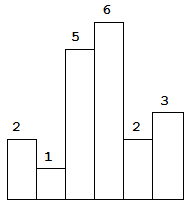
\includegraphics[width=150pt]{histogram.png}
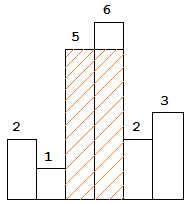
\includegraphics[width=150pt]{histogram2.png}
\end{center}

\subsubsection{Analysis}
\begin{Code}
这题关键是对于每根柱子,往两边延伸到某根柱子比自己矮或到边界为止。

暴力办法是依次循环,时间复杂度O(n^2),空间复杂度O(n)

采用动态规划延伸的时候可以根据之前的结果跳着走,最优时间复杂度O(n),最差时间复杂度O(n^2),
平均时间复杂度O(n),空间复杂度O(n)

采用压栈的方法最巧妙,时间复杂度O(n),空间复杂度O(n)
\end{Code}

\newpage

\subsubsection{Solution I}

\begin{Code}
// 这种超时了,复杂度O(n^2)
public int largestRectangleArea(int[] heights) {
    int max = 0;
    for (int i = 0, j, k; i < heights.length; i++) {
        for (j = i - 1; j >= 0 && heights[j] >= heights[i]; j--);
        for (k = i + 1; k < heights.length && heights[k] >= heights[i]; k++);
        max = Math.max(max, (k - j - 1) * heights[i]);
    }
    return max;
}

/** 注意栈中的是index,不是高度 */
public int largestRectangleArea2(int[] heights) {
    int max = 0;
    Stack<Integer> stack = new Stack<Integer>();
    for (int i = 0; i <= heights.length; ) {
        int height = i == heights.length ? 0 : heights[i];
        if (stack.isEmpty() || height > heights[stack.peek()]) {
            stack.push(i++);
        } else {
            int top = stack.pop();
            int left = stack.isEmpty() ? 0 : stack.peek() + 1;
            max = Math.max(max, heights[top] * (i - 1 - left + 1));
        }
    }
    return max;
}
\end{Code}

\subsubsection{Solution II}
\begin{Code}
// 耗时4ms
public int largestRectangleArea3(int[] heights) {
    int len = heights.length, j;
    int[] left = new int[len], right = new int[len];

    for (int i = 0; i < len; i++) {
        for (j = i; j >= 1 && heights[j - 1] >= heights[i]; j = left[j - 1]);
        left[i] = j;
    }

    for (int i = len - 1; i >= 0; i--) {
        for (j = i; j < len - 1 && heights[j + 1] >= heights[i]; j = right[j + 1]);
        right[i] = j;
    }

    int max = 0;
    for (int i = 0; i < len; i++) {
        max = Math.max(max, (right[i] - left[i] + 1) * heights[i]);
    }
    return max;
}
\end{Code}

\newpage

\section{Maximal Rectangle} %%%%%%%%%%%%%%%%%%%%%%



\subsubsection{Description}
Given a 2D binary matrix filled with 0's and 1's, find the largest rectangle containing only 1's and return its area.

For example, given the following matrix:
\begin{Code}
1 0 1 0 0
1 0 1 1 1
1 1 1 1 1
1 0 0 1 0
\end{Code}

Return 6.

\subsubsection{Solution I}

\begin{Code}
// 耗时10ms,时间复杂度是O(mn),空间复杂度O(n)
public int maximalRectangle(char[][] matrix) {
    if (matrix.length == 0) {
        return 0;
    }
    int row = matrix.length, col = matrix[0].length, max = 0;
    int[] heights = new int[col];
    for (int i = 0; i < row; i++) {
        for (int j = 0; j < col; j++) {
            if (matrix[i][j] == '0') {
                heights[j] = 0;
            } else {
                heights[j]++;
            }
        }
        max = Math.max(max, largestRectangleArea(heights));
    }
    return max;
}
\end{Code}

\newpage

\subsubsection{Solution II}
\begin{Code}
// 耗时9ms
public int maximalRectangle2(char[][] matrix) {
    if (matrix.length == 0) {
        return 0;
    }

    int row = matrix.length, col = matrix[0].length, area = 0;
    int[] height = new int[col], left = new int[col], right = new int[col];
    for (int i = 0; i < col; right[i] = col - 1, i++);

    for (int i = 0; i < row; i++) {
        int leftStart = 0, rightStart = col - 1;

        for (int j = 0; j < col; j++) {
            if (matrix[i][j] == '0') {
                height[j] = 0;
            } else {
                height[j]++;
            }
        }

        // 注意当matrix[i][j]为0时其实left[j]和right[j]是多少已经不重要了,因为
        // height[j]为0,所以这里算left[j]和right[j]只是为了方便计算下一层
        // 所以left[j]=0好理解,而right[j]=col-1的目的是为了设置成最大的,因为下一层要求min

        for (int j = 0; j < col; j++) {
            if (matrix[i][j] == '0') {
                left[j] = 0;
                leftStart = j + 1;
            } else {
                left[j] = Math.max(left[j], leftStart);
            }
        }

        for (int j = col - 1; j >= 0; j--) {
            // 注意这里不是0,而是字符'0'
            if (matrix[i][j] == '0') {
                right[j] = col - 1;
                rightStart = j - 1;
            } else {
                right[j] = Math.min(right[j], rightStart);
            }
        }

        for (int j = 0; j < col; j++) {
            area = Math.max(area, (right[j] - left[j] + 1) * height[j]);
        }
    }

    return area;
}
\end{Code}

\newpage

\section{Maximal Square} %%%%%%%%%%%%%%%%%%%%%%



\subsubsection{Description}
Given a 2D binary matrix filled with 0's and 1's, find the largest square containing only 1's and return its area.

For example, given the following matrix:
\begin{Code}
1 0 1 0 0
1 0 1 1 1
1 1 1 1 1
1 0 0 1 0
\end{Code}

Return 4.

\subsubsection{Solution}

\begin{Code}
/**
 * 这题要返回的是面积
 */
public int maximalSquare(char[][] matrix) {
    if (matrix == null || matrix.length == 0) {
        return 0;
    }

    int row = matrix.length, col = matrix[0].length;

    int[][] f = new int[row][col];

    int max = 0;

    for (int i = 0; i < col; i++) {
        f[0][i] = matrix[0][i] == '1' ? 1 : 0;
        max = Math.max(max, f[0][i]);
    }

    for (int i = 0; i < row; i++) {
        f[i][0] = matrix[i][0] == '1' ? 1 : 0;
        max = Math.max(max, f[i][0]);
    }

    for (int i = 1; i < row; i++) {
        for (int j = 1; j < col; j++) {
            if (matrix[i][j] == '0') {
                f[i][j] = 0;
            } else {
                int mn = Math.min(f[i - 1][j], f[i][j - 1]);
                f[i][j] = Math.min(mn, f[i - 1][j - 1]) + 1;
                max = Math.max(max, f[i][j]);
            }
        }
    }

    return max * max;
}
\end{Code}

\newpage

\section{Edit Distance} %%%%%%%%%%%%%%%%%%%%%%



\subsubsection{Description}
Given two words word1 and word2, find the minimum number of steps required to convert word1 to word2. (each operation is counted as 1 step.)

You have the following 3 operations permitted on a word:

a) Insert a character

b) Delete a character

c) Replace a character

\subsubsection{Solution}

\begin{Code}
public int minDistance(String word1, String word2) {
    int len1 = word1.length(), len2 = word2.length();
    int[][] f = new int[len1 + 1][len2 + 1];
    for (int i = 1; i <= len1; i++) {
        f[i][0] = i;
    }
    for (int i = 1; i <= len2; i++) {
        f[0][i] = i;
    }
    for (int i = 1; i <= len1; i++) {
        for (int j = 1; j <= len2; j++) {
            if (word1.charAt(i - 1) == word2.charAt(j - 1)) {
                f[i][j] = f[i - 1][j - 1];
            } else {
                int min = Math.min(f[i][j - 1], f[i - 1][j]);
                f[i][j] = Math.min(f[i - 1][j - 1], min) + 1; /** 这里的加1别掉了 */
            }
        }
    }
    return f[len1][len2];
}
\end{Code}

\newpage

\section{One Edit Distance} %%%%%%%%%%%%%%%%%%%%%%



\subsubsection{Description}
Given two strings S and T, determine if they are both one edit distance apart.

\subsubsection{Solution}

\begin{Code}
/**
 * 最容易错的是结尾的条件sL != tL
 */
public boolean isOneEditDistance(String s, String t) {
    int sL = s.length(), tL = t.length();
    if (sL > tL) {
        return isOneEditDistance(t, s);
    }
    if (tL - sL > 1) {
        return false;
    }

    for (int i = 0; i < sL; i++) {
        if (s.charAt(i) != t.charAt(i)) {
            if (sL < tL) {
                return s.substring(i).equals(t.substring(i + 1));
            } else {
                return s.substring(i + 1).equals(t.substring(i + 1));
            }
        }
    }
    return sL != tL;
}
\end{Code}

\newpage


\section{Distinct Subsequences} %%%%%%%%%%%%%%%%%%%%%%



\subsubsection{Description}
Given a string S and a string T, count the number of distinct subsequences of S which equals T.

A subsequence of a string is a new string which is formed from the original string by deleting some (can be none) of the characters without disturbing the relative positions of the remaining characters. (ie, "ACE" is a subsequence of "ABCDE" while "AEC" is not).

Here is an example:

S = \code{"rabbbit"}, T = \code{"rabbit"}

Return 3.

\subsubsection{Solution}

\begin{Code}

\end{Code}

\newpage

\section{Triangle} %%%%%%%%%%%%%%%%%%%%%%



\subsubsection{Description}
Given a triangle, find the minimum path sum from top to bottom. Each step you may move to adjacent numbers on the row below.

For example, given the following triangle
\begin{Code}
[
     [2],
    [3,4],
   [6,5,7],
  [4,1,8,3]
]
\end{Code}

The minimum path sum from top to bottom is 11 (i.e., 2 + 3 + 5 + 1 = 11).

\textbf{Note:}

Bonus point if you are able to do this using only O(n) extra space, where n is the total number of rows in the triangle.

\subsubsection{Solution}

\begin{Code}

\end{Code}

\newpage

\section{Perfect Squares} %%%%%%%%%%%%%%%%%%%%%%



\subsubsection{Description}
Given a positive integer n, find the least number of perfect square numbers (for example, 1, 4, 9, 16, ...) which sum to n.

For example, given n = 12, return 3 because 12 = 4 + 4 + 4; given n = 13, return 2 because 13 = 4 + 9.

\subsubsection{Solution}

\begin{Code}
public int numSquares(int n) {
    int[] dp = new int[n + 1];
    for (int i = 1; i <= n; i++) {
        int min = Integer.MAX_VALUE;
        for (int k = 1; i - k * k >= 0; k++) {
            min = Math.min(min, 1 + dp[i - k * k]);
        }
        dp[i] = min;
    }
    return dp[n];
}
\end{Code}

\newpage

\section{Range Sum Query - Immutable} %%%%%%%%%%%%%%%%%%%%%%



\subsubsection{Description}

Given an integer array nums, find the sum of the elements between indices i and j (i ≤ j), inclusive.

\textbf{Example:}

Given nums = [-2, 0, 3, -5, 2, -1]

sumRange(0, 2) -> 1

sumRange(2, 5) -> -1

sumRange(0, 5) -> -3

\textbf{Note:}

You may assume that the array does not change.

There are many calls to sumRange function.

\subsubsection{Solution}

\begin{Code}
private int[] sums;

public RangeSumQueryImmutable(int[] nums) {
    sums = new int[nums.length];
    for (int sum = 0, i = 0; i < nums.length; i++) {
        sum += nums[i];
        sums[i] = sum;
    }
}

public int sumRange(int i, int j) {
    int sum1 = i > 0 ? sums[i - 1] : 0;
    return sums[j] - sum1;
}
\end{Code}

\newpage

\section{Range Sum Query 2D - Immutable} %%%%%%%%%%%%%%%%%%%%%%



\subsubsection{Description}
Given a 2D matrix matrix, find the sum of the elements inside the rectangle defined by its upper left corner (row1, col1) and lower right corner (row2, col2).

\begin{center}
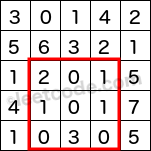
\includegraphics[width=60pt]{range.png}
\end{center}

\textbf{Example:}
\begin{Code}
Given matrix = [
  [3, 0, 1, 4, 2],
  [5, 6, 3, 2, 1],
  [1, 2, 0, 1, 5],
  [4, 1, 0, 1, 7],
  [1, 0, 3, 0, 5]
]

sumRegion(2, 1, 4, 3) -> 8, sumRegion(1, 1, 2, 2) -> 11, sumRegion(1, 2, 2, 4) -> 12
\end{Code}

\textbf{Note:}

1. You may assume that the matrix does not change.

2. There are many calls to sumRegion function.

3. You may assume that row1 ≤ row2 and col1 ≤ col2.

\subsubsection{Solution}

\begin{Code}
public class solution.NumMatrix {
    private int[][] dp;

    public solution.NumMatrix(int[][] matrix) {
        if (matrix.length == 0) {
            return;
        }
        int row = matrix.length;
        int col = matrix[0].length;
        dp = new int[row + 1][col + 1];

        for (int i = 1; i <= row; i++) {
            for (int j = 1; j <= col; j++) {
                dp[i][j] = dp[i - 1][j] + dp[i][j - 1] - dp[i - 1][j - 1] + matrix[i - 1][j - 1];
            }
        }
    }

    public int sumRegion(int row1, int col1, int row2, int col2) {
        return dp[row2 + 1][col2 + 1] - dp[row2 + 1][col1] - dp[row1][col2 + 1] + dp[row1][col1];
    }
}
\end{Code}

\newpage

\section{Unique Paths} %%%%%%%%%%%%%%%%%%%%%%



\subsubsection{Description}
A robot is located at the top-left corner of a m x n grid (marked 'Start' in the diagram below).

The robot can only move either down or right at any point in time. The robot is trying to reach the bottom-right corner of the grid (marked 'Finish' in the diagram below).

How many possible unique paths are there?

\begin{center}
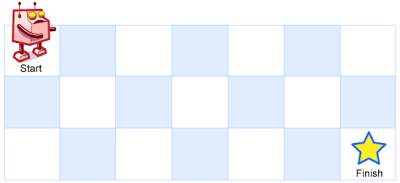
\includegraphics[width=100pt]{robot.png}\\
\end{center}

\textbf{Note:} m and n will be at most 100.

\subsubsection{Solution}

\begin{Code}

\end{Code}

\newpage

\section{Unique Paths II} %%%%%%%%%%%%%%%%%%%%%%



\subsubsection{Description}
Follow up for "Unique Paths":

Now consider if some obstacles are added to the grids. How many unique paths would there be?

An obstacle and empty space is marked as 1 and 0 respectively in the grid.

For example,

There is one obstacle in the middle of a 3x3 grid as illustrated below.
\begin{Code}
[
  [0,0,0],
  [0,1,0],
  [0,0,0]
]
\end{Code}

The total number of unique paths is 2.

\textbf{Note:} m and n will be at most 100.

\subsubsection{Solution}

\begin{Code}

\end{Code}

\newpage

\section{Burst Balloons} %%%%%%%%%%%%%%%%%%%%%%



\subsubsection{Description}
Given n balloons, indexed from 0 to n-1. Each balloon is painted with a number on it represented by array nums. You are asked to burst all the balloons. If the you burst balloon i you will get nums[left] * nums[i] * nums[right] coins. Here left and right are adjacent indices of i. After the burst, the left and right then becomes adjacent.

Find the maximum coins you can collect by bursting the balloons wisely.

\textbf{Note:}

(1) You may imagine nums[-1] = nums[n] = 1. They are not real therefore you can not burst them.

(2) 0 ≤ n ≤ 500, 0 ≤ nums[i] ≤ 100

\textbf{Example:}

Given [3, 1, 5, 8]

Return 167
\begin{Code}
    nums = [3,1,5,8] --> [3,5,8] -->   [3,8]   -->  [8]  --> []
   coins =  3*1*5      +  3*5*8    +  1*3*8      + 1*8*1   = 167
\end{Code}
\subsubsection{Solution}

\begin{Code}
/**
 * 这题用的闭区间DP,dp[start][end]表示区间start,end内所有气球爆掉的最大coin
 * 假设最后爆第i个气球,start <= i <= end,则对应的coin为
 * coin = nums[start - 1] * nums[i] * nums[end + 1] + dp[start, i - 1] + dp[i + 1][end]
 * 为什么最后爆呢,因为这样以i为分隔线的左右两边就相互独立了,否则如果先爆i,则i的左右两个气球就相邻了
 * 为什么最后爆i时,其相邻值取nums[start - 1]和nums[end + 1]呢?放在全局来看,
 * 就是nums[-1]和nums[n]都为1
 */
public int maxCoins(int[] nums) {
    if (nums.length == 0) {return 0;}

    int n = nums.length;
    int[][] dp = new int[n][n];
    for (int len = 1; len <= n; len++) {
        for (int start = 0; start + len - 1 < n; start++) {
            int end = start + len - 1;
            for (int i = start; i <= end; i++) {
                int coins = nums[i] * getValue(nums, start - 1) * getValue(nums, end + 1);
                coins += i > start ? dp[start][i - 1] : 0;
                coins += i < end ? dp[i + 1][end] : 0;
                dp[start][end] = Math.max(dp[start][end], coins);
            }
        }
    }
    return dp[0][n - 1];
}

private int getValue(int[] nums, int i) {
    if (i < 0 || i >= nums.length) {
        return 1;
    }
    return nums[i];
}
\end{Code}

\newpage

\section{Minimum Path Sum} %%%%%%%%%%%%%%%%%%%%%%



\subsubsection{Description}
Given a m x n grid filled with non-negative numbers, find a path from top left to bottom right which minimizes the sum of all numbers along its path.

\textbf{Note:} You can only move either down or right at any point in time.

\subsubsection{Solution}

\begin{Code}

\end{Code}

\newpage

\section{Decode Ways} %%%%%%%%%%%%%%%%%%%%%%



\subsubsection{Description}
A message containing letters from A-Z is being encoded to numbers using the following mapping:
\begin{Code}
'A' -> 1
'B' -> 2
...
'Z' -> 26
\end{Code}
Given an encoded message containing digits, determine the total number of ways to decode it.

For example,

Given encoded message "12", it could be decoded as "AB" (1 2) or "L" (12).

The number of ways decoding "12" is 2.
\subsubsection{Solution}

\begin{Code}
// DP,耗时2ms,复杂度O(n)
public int numDecodings2(String s) {
    if (s.length() == 0) {
        return 0;
    }
    int n = s.length();
    int[] f = new int[n + 1];
    f[0] = 1;
    f[1] = s.charAt(0) == '0' ? 0 : 1;

    for (int i = 1; i < n; i++) {
        if (s.charAt(i - 1) == '1' || (s.charAt(i - 1) == '2' && s.charAt(i) <= '6')) {
            f[i + 1] = f[i - 1];
        }
        if (s.charAt(i) != '0') {
            f[i + 1] += f[i];
        }
    }
    return f[n];
}
\end{Code}

\newpage

\section{Decode Ways II} %%%%%%%%%%%%%%%%%%%%%%



\subsubsection{Description}
A message containing letters from A-Z is being encoded to numbers using the following mapping way:
\begin{Code}
'A' -> 1
'B' -> 2
...
'Z' -> 26
\end{Code}

Beyond that, now the encoded string can also contain the character '*', which can be treated as one of the numbers from 1 to 9.

Given the encoded message containing digits and the character '*', return the total number of ways to decode it.

Also, since the answer may be very large, you should return the output mod 109 + 7.

\textbf{Example 1:}

\textbf{Input:} \code{"*"}

\textbf{Output:} 9

\textbf{Explanation:} The encoded message can be decoded to the string: \code{"A", "B", "C", "D", "E", "F", "G", "H", "I"}.

\textbf{Example 2:}

\textbf{Input:} \code{"1*"}

\textbf{Output:} 9 + 9 = 18

\textbf{Note:}

The length of the input string will fit in range [1, 105].

The input string will only contain the character \code{'*'} and digits \code{'0' - '9'}.
\subsubsection{Solution}

\begin{Code}

\end{Code}

\newpage

\section{Scramble String} %%%%%%%%%%%%%%%%%%%%%%



\subsubsection{Description}
Given a string s1, we may represent it as a binary tree by partitioning it to two non-empty substrings recursively.

Below is one possible representation of s1 = \code{"great"}:
\begin{Code}
    great
   /    \
  gr    eat
 / \    /  \
g   r  e   at
           / \
          a   t
\end{Code}
To scramble the string, we may choose any non-leaf node and swap its two children.

For example, if we choose the node "gr" and swap its two children, it produces a scrambled string "rgeat".
\begin{Code}
    rgeat
   /    \
  rg    eat
 / \    /  \
r   g  e   at
           / \
          a   t
\end{Code}
We say that "rgeat" is a scrambled string of "great".

Similarly, if we continue to swap the children of nodes "eat" and "at", it produces a scrambled string "rgtae".
\begin{Code}
    rgtae
   /    \
  rg    tae
 / \    /  \
r   g  ta  e
       / \
      t   a
\end{Code}
We say that "rgtae" is a scrambled string of "great".

Given two strings s1 and s2 of the same length, determine if s2 is a scrambled string of s1.
\subsubsection{Solution}

\begin{Code}

\end{Code}

\newpage

\section{Interleaving String} %%%%%%%%%%%%%%%%%%%%%%



\subsubsection{Description}
Given s1, s2, s3, find whether s3 is formed by the interleaving of s1 and s2.

For example,

Given:
\begin{Code}
s1 = "aabcc",
s2 = "dbbca",

When s3 = "aadbbcbcac", return true.
When s3 = "aadbbbaccc", return false.
\end{Code}
\subsubsection{Solution}

\begin{Code}

\end{Code}

\newpage


\section{Coin Change} %%%%%%%%%%%%%%%%%%%%%%



\subsubsection{Description}
You are given coins of different denominations and a total amount of money amount. Write a function to compute the fewest number of coins that you need to make up that amount. If that amount of money cannot be made up by any combination of the coins, return -1.

\textbf{Example 1:}
coins = [1, 2, 5], amount = 11

return 3 (11 = 5 + 5 + 1)

\textbf{Example 2:}

coins = [2], amount = 3

return -1.

\textbf{Note:}

You may assume that you have an infinite number of each kind of coin.

\subsubsection{Solution}

\begin{Code}

\end{Code}

\newpage

\section{Ugly Number II} %%%%%%%%%%%%%%%%%%%%%%



\subsubsection{Description}
Write a program to find the n-th ugly number.

Ugly numbers are positive numbers whose prime factors only include 2, 3, 5. For example, 1, 2, 3, 4, 5, 6, 8, 9, 10, 12 is the sequence of the first 10 ugly numbers.

Note that 1 is typically treated as an ugly number, and n does not exceed 1690.

\subsubsection{Solution}

\begin{Code}
public int nthUglyNumber(int n) {
    int[] f = new int[n];
    f[0] = 1;
    int t2 = 0, t3 = 0, t5 = 0;
    for (int i = 1; i < n; i++) {
        f[i] = Math.min(Math.min(f[t2] * 2, f[t3] * 3), f[t5] * 5);

        if(f[i] >= f[t2] * 2) {
            t2++;
        }
        if(f[i] >= f[t3] * 3) {
            t3++;
        }
        if(f[i] >= f[t5] * 5) {
            t5++;
        }
    }
    return f[n - 1];
}
\end{Code}

\newpage

\section{Integer Break} %%%%%%%%%%%%%%%%%%%%%%



\subsubsection{Description}
Given a positive integer n, break it into the sum of at least two positive integers and maximize the product of those integers. Return the maximum product you can get.

For example, given n = 2, return 1 (2 = 1 + 1); given n = 10, return 36 (10 = 3 + 3 + 4).

\textbf{Note:} You may assume that n is not less than 2 and not larger than 58.

\subsubsection{Solution}

\begin{Code}

\end{Code}

\newpage

\section{Longest Valid Parentheses} %%%%%%%%%%%%%%%%%%%%%%



\subsubsection{Description}
Given a string containing just the characters '(' and ')', find the length of the longest valid (well-formed) parentheses substring.

For "(()", the longest valid parentheses substring is "()", which has length = 2.

Another example is ")()())", where the longest valid parentheses substring is "()()", which has length = 4.

\subsubsection{Solution}

\begin{Code}
public int longestValidParentheses(String s) {
    Stack<Integer> stack = new Stack<Integer>();
    for (int i = 0; i < s.length(); i++) {
        if (s.charAt(i) == ')' && !stack.isEmpty() && s.charAt(stack.peek()) == '(') {
            stack.pop();
        } else {
            stack.push(i);
        }
    }

    int max = 0, cur = s.length();
    while (!stack.isEmpty()) {
        int prev = stack.pop();
        /**
         * (prev, cur)之间是合法部分,注意左右都是开区间
         */
        max = Math.max(cur - prev - 1, max);
        cur = prev;
    }

    /**
     * 栈空了,表示最后一个栈顶的左边都是合法部分了,即[0,end)之间是合法部分,这部分也要参与计算
     */
    return Math.max(max, cur);
}
\end{Code}

\newpage

\section{Longest Increasing Subsequence} %%%%%%%%%%%%%%%%%%%%%%



\subsubsection{Description}
Given an unsorted array of integers, find the length of longest increasing subsequence.

For example,

Given [10, 9, 2, 5, 3, 7, 101, 18],

The longest increasing subsequence is [2, 3, 7, 101], therefore the length is 4. Note that there may be more than one LIS combination, it is only necessary for you to return the length.

Your algorithm should run in O(n2) complexity.

\textbf{Follow up:} Could you improve it to O(n log n) time complexity?

\subsubsection{Solution I}

\begin{Code}
/**
 * 这题是典型的DP,f[i]包含i的最长子序列长度
 */
public int lengthOfLIS(int[] nums) {
    int n = nums.length;
    if (n == 0) {
        return 0;
    }
    int[] f = new int[n];
    /**
     * 注意这里fill是有必要的
     */
    Arrays.fill(f, 1);
    int max = 1;
    for (int i = 1; i < n; i++) {
        for (int j = 0; j < i; j++) {
            if (nums[i] > nums[j]) {
                f[i] = Math.max(f[i], f[j] + 1);
            }
        }
        max = Math.max(max, f[i]);
    }
    return max;
}
\end{Code}

\newpage

\subsubsection{Solution II}
\begin{Code}
public int lengthOfLIS2(int[] nums) {
    int len = 1;
    for (int i = 0; i < nums.length; i++) {
        /**
         * 注意这里要指定区间,且end是开区间
         */
        int k = Arrays.binarySearch(nums, 0, len, nums[i]);
        /**
         * 只处理k<0的情况
         */
        if (k < 0) {
            k = -(k + 1);
            if (k == len) {
                len++;
            }
            nums[k] = nums[i];
        }
    }
    return len;
}
\end{Code}

\newpage

\section{Count Numbers with Unique Digits} %%%%%%%%%%%%%%%%%%%%%%



\subsubsection{Description}
Given a non-negative integer n, count all numbers with unique digits, x, where 0 ≤ x < 10n.

\textbf{Example:}

Given n = 2, return 91. (The answer should be the total numbers in the range of 0 ≤ x < 100, excluding [11,22,33,44,55,66,77,88,99])

\subsubsection{Solution}

\begin{Code}
public int countNumbersWithUniqueDigits(int n) {
    int[] result = new int[n + 1];
    result[0] = 1;
    for (int i = 1, t = 9; i <= n; i++) {
        result[i] = result[i - 1] + t;
        t *= 10 - i;
    }
    return result[n];
}
\end{Code}

\newpage

\section{Create Maximum Number} %%%%%%%%%%%%%%%%%%%%%%



\subsubsection{Description}
Given two arrays of length m and n with digits 0-9 representing two numbers. Create the maximum number of length k <= m + n from digits of the two. The relative order of the digits from the same array must be preserved. Return an array of the k digits. You should try to optimize your time and space complexity.

\textbf{Example 1:}

nums1 = [3, 4, 6, 5]

nums2 = [9, 1, 2, 5, 8, 3]

k = 5

return [9, 8, 6, 5, 3]

\textbf{Example 2:}

nums1 = [6, 7]

nums2 = [6, 0, 4]

k = 5

return [6, 7, 6, 0, 4]

\textbf{Example 3:}

nums1 = [3, 9]

nums2 = [8, 9]

k = 3

return [9, 8, 9]
\subsubsection{Solution}

\begin{Code}

\end{Code}

\newpage

\section{Guess Number Higher or Lower II} %%%%%%%%%%%%%%%%%%%%%%



\subsubsection{Description}
We are playing the Guess Game. The game is as follows:

I pick a number from 1 to n. You have to guess which number I picked.

Every time you guess wrong, I'll tell you whether the number I picked is higher or lower.

However, when you guess a particular number x, and you guess wrong, you pay x. You win the game when you guess the number I picked.

\textbf{Example:}

n = 10, I pick 8.

First round:  You guess 5, I tell you that it's higher. You pay 5.

Second round: You guess 7, I tell you that it's higher. You pay 7.

Third round:  You guess 9, I tell you that it's lower. You pay 9.

Game over. 8 is the number I picked.

You end up paying 5 + 7 + 9 = 21.

Given a particular n ≥ 1, find out how much money you need to have to guarantee a win.
\subsubsection{Solution I}

\begin{Code}
/**
 * 在[start,end]中首先挑i,最差情况是i是错的,那么cost要加i,然后再从[start,i-1]和[i+1,end]中
 * 继续挑,由于是最差情况,所以我们假定每次都是错的,
 * 所以cost(start,end)=i+max(cost(start,i-1),cost(i+1,end)),
 * i在[start,end]之间遍历,从所有最差情况中找到一个最小值,这就是我们要首先猜的那个数了。
 */

public int getMoneyAmount(int n) {
    return getMoneyAmount(1, n);
}

// 暴力方法,时间复杂度O(n!), 空间复杂度O(n)
private int getMoneyAmount(int start, int end) {
    if (start >= end) {
        return 0;
    }
    int min = Integer.MAX_VALUE;
    for (int i = start; i <= end; i++) {
        int res = i + Math.max(getMoneyAmount(start, i - 1), getMoneyAmount(i + 1, end));
        min = Math.min(min, res);
    }
    return min;
}
\end{Code}

\newpage

\subsubsection{Solution II}
\begin{Code}
// 耗时18ms,和上面思路一样,只是用了缓存,避免重复计算
public int getMoneyAmount(int n) {
    int[][] dp = new int[n + 1][n + 1];
    return getMoneyAmount(dp, 1, n);
}

private int getMoneyAmount(int[][] dp, int start, int end) {
    if (start >= end) {
        return 0;
    }
    if (dp[start][end] != 0) {
        return dp[start][end];
    }
    int min = Integer.MAX_VALUE;
    for (int i = start; i <= end; i++) {
        int res = i + Math.max(getMoneyAmount(dp, start, i - 1), getMoneyAmount(dp, i + 1, end));
        min = Math.min(min, res);
    }
    dp[start][end] = min;
    return min;
}
\end{Code}

\subsubsection{Solution III}
\begin{Code}
// 注意这里len要从2开始,耗时15ms
public int getMoneyAmount(int n) {
    int[][] dp = new int[n + 1][n + 1];
    for (int len = 2; len <= n; len++) {

        for (int start = 1; start + len - 1 <= n; start++) {
            int minRes = Integer.MAX_VALUE;

            // 注意这里pivot的边界,因为下面有pivot+1可能越界
            for (int pivot = start; pivot < start + len - 1; pivot++) {
                int res = pivot + Math.max(dp[start][pivot - 1], dp[pivot + 1][start + len - 1]);
                minRes = Math.min(res, minRes);
            }

            dp[start][start + len - 1] = minRes;
        }
    }
    return dp[1][n];
}

/**
 * 还有一点优化,不过我没想太明白,就是选择pivot时,以(start+end)/2为起点,而不是从start,大致原因是
 * 相同长度下,数字越小的序列试错成本越低,所以以左边为轴的试错成本肯定高于以右边为轴的成本。
 */
\end{Code}

\newpage

\section{Paint House} %%%%%%%%%%%%%%%%%%%%%%



\subsubsection{Description}
There are a row of n houses, each house can be painted with one of the three colors: red, blue or green. The cost of painting each house with a certain color is different. You have to paint all the houses such that no two adjacent houses have the same color.

The cost of painting each house with a certain color is represented by a n x 3 cost matrix. For example, costs[0][0] is the cost of painting house 0 with color red; costs[1][2] is the cost of painting house 1 with color green, and so on... Find the minimum cost to paint all houses.

\textbf{Note:}

All costs are positive integers.

\subsubsection{Solution}

\begin{Code}
public int minCost(int[][] costs) {
    int[] f = new int[3];
    int f0 = 0, f1 = 0, f2 = 0;
    for (int i = 0; i < costs.length; i++) {
        f[0] = costs[i][0] + Math.min(f1, f2);
        f[1] = costs[i][1] + Math.min(f0, f2);
        f[2] = costs[i][2] + Math.min(f0, f1);
        f0 = f[0]; f1 = f[1]; f2 = f[2];
    }
    return Math.min(Math.min(f0, f1), f2);
}
\end{Code}

\newpage

\section{Paint House II} %%%%%%%%%%%%%%%%%%%%%%



\subsubsection{Description}
There are a row of n houses, each house can be painted with one of the k colors. The cost of painting each house with a certain color is different. You have to paint all the houses such that no two adjacent houses have the same color.

The cost of painting each house with a certain color is represented by a n x k cost matrix. For example, costs[0][0] is the cost of painting house 0 with color 0; costs[1][2] is the cost of painting house 1 with color 2, and so on... Find the minimum cost to paint all houses.

\textbf{Note:}

All costs are positive integers.

\textbf{Follow up:}

Could you solve it in O(nk) runtime?

\subsubsection{Solution}

\begin{Code}
/**
 * 思路很简单,只要记录上一个house为止的最小cost及index以及次小cost即可
 * 遍历当前house的各种颜色,如果当前颜色和上个house最小cost的颜色不同,则上个house可以取最小cost,否则取次小cost
 */
public int minCostII(int[][] costs) {
    if (costs.length == 0) {
        return 0;
    }
    int k = costs[0].length;
    int min = 0, minIdx = -1, submin = 0;
    for (int i = 0; i < costs.length; i++) {
        int min0 = Integer.MAX_VALUE, minIdx0 = -1, submin0 = Integer.MAX_VALUE;
        for (int j = 0; j < k; j++) {
            int cost = costs[i][j] + (j != minIdx ? min : submin);
            if (cost < min0) {
                submin0 = min0;
                min0 = cost;
                minIdx0 = j;
            } else if (cost < submin0) {
                submin0 = cost;
            }
        }
        min = min0; minIdx = minIdx0; submin = submin0;
    }
    return min;
}
\end{Code}

\newpage

\section{Russian Doll Envelopes} %%%%%%%%%%%%%%%%%%%%%%



\subsubsection{Description}
You have a number of envelopes with widths and heights given as a pair of integers (w, h). One envelope can fit into another if and only if both the width and height of one envelope is greater than the width and height of the other envelope.

What is the maximum number of envelopes can you Russian doll? (put one inside other)

\textbf{Example:}
\begin{Code}
Given envelopes = [[5,4],[6,4],[6,7],[2,3]], the maximum number of envelopes you can Russian doll is 3 ([2,3] => [5,4] => [6,7]).
\end{Code}

\subsubsection{Solution}

\begin{Code}

\end{Code}

\newpage

\section{Max Sum of Rectangle No Larger Than K} %%%%%%%%%%%%%%%%%%%%%%



\subsubsection{Description}
Given a non-empty 2D matrix matrix and an integer k, find the max sum of a rectangle in the matrix such that its sum is no larger than k.

\textbf{Example:}
\begin{Code}
Given matrix = [
  [1,  0, 1],
  [0, -2, 3]
]
\end{Code}

k = 2

The answer is 2. Because the sum of rectangle [[0, 1], [-2, 3]] is 2 and 2 is the max number no larger than k (k = 2).

\textbf{Note:}

1. The rectangle inside the matrix must have an area > 0.

2. What if the number of rows is much larger than the number of columns?

\subsubsection{Solution}

\begin{Code}

\end{Code}

\newpage

\section{Wiggle Subsequence} %%%%%%%%%%%%%%%%%%%%%%



\subsubsection{Description}
A sequence of numbers is called a wiggle sequence if the differences between successive numbers strictly alternate between positive and negative. The first difference (if one exists) may be either positive or negative. A sequence with fewer than two elements is trivially a wiggle sequence.

For example, [1,7,4,9,2,5] is a wiggle sequence because the differences (6,-3,5,-7,3) are alternately positive and negative. In contrast, [1,4,7,2,5] and [1,7,4,5,5] are not wiggle sequences, the first because its first two differences are positive and the second because its last difference is zero.

Given a sequence of integers, return the length of the longest subsequence that is a wiggle sequence. A subsequence is obtained by deleting some number of elements (eventually, also zero) from the original sequence, leaving the remaining elements in their original order.

\textbf{Examples:}

\textbf{Input:} [1,7,4,9,2,5]

\textbf{Output:} 6

The entire sequence is a wiggle sequence.

\textbf{Input:} [1,17,5,10,13,15,10,5,16,8]

\textbf{Output:} 7

There are several subsequences that achieve this length. One is [1,17,10,13,10,16,8].

\textbf{Input:} [1,2,3,4,5,6,7,8,9]

\textbf{Output:} 2

\textbf{Follow up:}

Can you do it in O(n) time?

\subsubsection{Solution}

\begin{Code}

\end{Code}

\newpage

\section{Largest Divisible Subset} %%%%%%%%%%%%%%%%%%%%%%



\subsubsection{Description}
Given a set of distinct positive integers, find the largest subset such that every pair (Si, Sj) of elements in this subset satisfies: Si % Sj = 0 or Sj % Si = 0.

If there are multiple solutions, return any subset is fine.

\textbf{Example 1:}

nums: [1,2,3]

Result: [1,2] (of course, [1,3] will also be ok)

\textbf{Example 2:}

nums: [1,2,4,8]

Result: [1,2,4,8]
\subsubsection{Solution}

\begin{Code}

\end{Code}

\newpage

\section{Paint Fence} %%%%%%%%%%%%%%%%%%%%%%



\subsubsection{Description}
There is a fence with n posts, each post can be painted with one of the k colors.

You have to paint all the posts such that no more than two adjacent fence posts have the same color.

Return the total number of ways you can paint the fence.

\textbf{Note:}

n and k are non-negative integers.

\subsubsection{Solution}

\begin{Code}

\end{Code}

\newpage

\section{Bomb Enemy} %%%%%%%%%%%%%%%%%%%%%%



\subsubsection{Description}
Given a 2D grid, each cell is either a wall 'W', an enemy 'E' or empty '0' (the number zero), return the maximum enemies you can kill using one bomb.

The bomb kills all the enemies in the same row and column from the planted point until it hits the wall since the wall is too strong to be destroyed.

Note that you can only put the bomb at an empty cell.

\textbf{Example:}

For the given grid
\begin{Code}
0 E 0 0
E 0 W E
0 E 0 0
\end{Code}

return 3. (Placing a bomb at (1,1) kills 3 enemies)

\newpage

\subsubsection{Solution}

\begin{Code}
public int maxKilledEnemies(char[][] grid) {
    if (grid.length == 0) {
        return 0;
    }

    int row = grid.length, col = grid[0].length;

    int result = 0, rowhits = 0;
    int[] colhits = new int[col];

    for (int i = 0; i < row; i++) {
        // 这个循环里每次都从墙或边界开始,是为了避免重复计算
        for (int j = 0; j < col; j++) {
            /** 如果当前是墙则直接跳过 */
            if (grid[i][j] == 'W') {
                continue;
            }

            // rowhits表示在当前点横向能杀伤的人数
            // 如果左边靠着墙或边界则统计往右延伸能杀多少敌人
            // 如果不是靠着墙,则不用统计了,直接复用本行之前的结果
            if (j == 0 || grid[i][j - 1] == 'W') {
                /** 注意这里rowhits要清零 */
                rowhits = 0;
                // 往右延伸一直到墙或边界
                for (int k = j; k < col && grid[i][k] != 'W'; k++) {
                    rowhits += (grid[i][k] == 'E') ? 1 : 0;
                }
            }

            // colhits表示本行第j列纵向能杀伤的人数
            // 如果上面靠着墙或边界则统计往下延伸能杀伤多少人
            // 如果不是靠着墙则不用统计了,直接复用本列之前的结果
            if (i == 0 || grid[i - 1][j] == 'W') {
                /** 注意这里colhits[j]要清零 */
                colhits[j] = 0;
                // 往下延伸到边界或者墙
                for (int k = i; k < row && grid[k][j] != 'W'; k++) {
                    colhits[j] += (grid[k][j] == 'E') ? 1 : 0;
                }
            }

            // 如果当前可以放炸弹,横向和纵向总杀伤人数和
            /** 这里要判断是否可以放炸弹 */
            if (grid[i][j] == '0') {
                result = Math.max(result, rowhits + colhits[j]);
            }
        }
    }

    return result;
}
\end{Code}

\newpage

\section{Is Subsequence} %%%%%%%%%%%%%%%%%%%%%%



\subsubsection{Description}
Given a string s and a string t, check if s is subsequence of t.

You may assume that there is only lower case English letters in both s and t. t is potentially a very long (length ~= 500,000) string, and s is a short string (<=100).

A subsequence of a string is a new string which is formed from the original string by deleting some (can be none) of the characters without disturbing the relative positions of the remaining characters. (ie, "ace" is a subsequence of "abcde" while "aec" is not).

\textbf{Example 1:}

s = \code{"abc"}, t = \code{"ahbgdc"}

Return true.

\textbf{Example 2:}

s = \code{"axc"}, t = \code{"ahbgdc"}

Return false.

\textbf{Follow up:}

If there are lots of incoming S, say S1, S2, ... , Sk where k >= 1B, and you want to check one by one to see if T has its subsequence. In this scenario, how would you change your code?
\subsubsection{Solution}

\begin{Code}

\end{Code}

\newpage

\section{Sentence Screen Fitting} %%%%%%%%%%%%%%%%%%%%%%



\subsubsection{Description}
Given a rows x cols screen and a sentence represented by a list of non-empty words, find how many times the given sentence can be fitted on the screen.

\textbf{Note:}

1. A word cannot be split into two lines.

2. The order of words in the sentence must remain unchanged.

3. Two consecutive words in a line must be separated by a single space.

4. Total words in the sentence won't exceed 100.

5. Length of each word is greater than 0 and won't exceed 10.

6. 1 ≤ rows, cols ≤ 20,000.

\textbf{Example 1:}

\textbf{Input:}

rows = 2, cols = 8, sentence = \code{["hello", "world"]}

\textbf{Output:}
1

\textbf{Explanation:}

hello---

world---

The character '-' signifies an empty space on the screen.

\textbf{Example 2:}

\textbf{Input:}

rows = 3, cols = 6, sentence = \code{["a", "bcd", "e"]}

\textbf{Output:}
2

\textbf{Explanation:}
\begin{Code}
a-bcd-
e-a---
bcd-e-
\end{Code}

The character '-' signifies an empty space on the screen.

\textbf{Example 3:}

\textbf{Input:}

rows = 4, cols = 5, sentence = ["I", "had", "apple", "pie"]

\textbf{Output:}
1

\textbf{Explanation:}
\begin{Code}
I-had
apple
pie-I
had--
\end{Code}

The character '-' signifies an empty space on the screen.

\newpage

\subsubsection{Solution}

\begin{Code}

\end{Code}

\newpage

\section{Split Array Largest Sum} %%%%%%%%%%%%%%%%%%%%%%



\subsubsection{Description}
Given an array which consists of non-negative integers and an integer m, you can split the array into m non-empty continuous subarrays. Write an algorithm to minimize the largest sum among these m subarrays.

\textbf{Note:}

If n is the length of array, assume the following constraints are satisfied:

1 ≤ n ≤ 1000

1 ≤ m ≤ min(50, n)

\textbf{Examples:}

\textbf{Input:}

nums = [7,2,5,10,8]

m = 2

\textbf{Output:}

18

\textbf{Explanation:}

There are four ways to split nums into two subarrays.

The best way is to split it into [7,2,5] and [10,8],

where the largest sum among the two subarrays is only 18.

\subsubsection{Analysis}
将数组切成m段,求所有段中最大值的最小值

我们倒过来思考,假设这个值为k,则意味着所有段的和都不会超过k,如果我们能确保这种情况下数组能被切成m段,则表明k是候选的值。那怎样确保k是最小值呢?

简单的办法是让k从最小开始,依次递增,k最小是多少呢,如果不考虑具体的m,显然是数组中的最大值,而k的最大值是整个数组的和。现在我们考虑m,如果k设置的太小,

则为了保证所有段的和都小于k,势必段要缩短长度以降低sum,而这样的话可能段的个数会超过m。如果k设置的太大,则势必段的长度要增加,而这样的话可能段的个数会达不到m,

所以k和m是线性关系,为了找到最小的那个k,我们可以用二分查找法。

\newpage

\subsubsection{Solution I}

\begin{Code}
/**
 * 这里二分查找时关键要注意的是只剩两个数时的情况,即r-l=1时,
 * 假设最终结果是l,则mid为l,isTargetBig返回true,所以返回l
 * 如果最终结果是r,则mid为l,isTargetBig返回false,所以l=mid+1=r,返回r
 */
public int splitArray(int[] nums, int m) {
    int max = 0, sum = 0;
    for (int i = 0; i < nums.length; i++) {
        max = Math.max(max, nums[i]);
        sum += nums[i];
    }
    int l = max, r = sum;
    while (l <= r) {
        int mid = l + ((r - l) >>> 1);
        if (isTargetBig(mid, nums, m)) {
            r = mid - 1;
        } else {
            l = mid + 1;
        }
    }
    return l;
}

/**
 *  如果target小了则返回false,正常或者大了则返回true
 */
private boolean isTargetBig(int target, int[] nums, int m) {
    int sum = 0, count = 1;
    for (int i = 0; i < nums.length; i++) {
        sum += nums[i];
        if (sum > target) {
            sum = nums[i];
            if (++count > m) {
                return false;
            }
        }
    }
    return true;
}
\end{Code}

\newpage

\subsubsection{Solution II}
\begin{Code}
/** 这种写法好理解一些,注意count==m时,也要缩小右边界,因为我们要找到尽可能小的值,
 * 假如mid恰好就是最小的值,之后left会加回来的
 */
public int splitArray(int[] nums, int m) {
    int max = 0, sum = 0;
    for (int n : nums) {
        max = Math.max(max, n);
        sum += n;
    }
    int left = max, right = sum;
    while (left <= right) {
        int mid = left + (right - left) / 2;
        int count = getCount(nums, mid);
        if (count > m) {
            left = mid + 1;
        } else if (count <= m) {
            right = mid - 1;
        }
    }
    return left;
}

private int getCount(int[] nums, int k) {
    int sum = 0, count = 1;
    for (int i = 0; i < nums.length; i++) {
        sum += nums[i];
        if (sum > k) {
            count++;
            sum = nums[i];
        }
    }
    return count;
}*/
\end{Code}

\newpage

\section{Partition Equal Subset Sum} %%%%%%%%%%%%%%%%%%%%%%



\subsubsection{Description}
Given a non-empty array containing only positive integers, find if the array can be partitioned into two subsets such that the sum of elements in both subsets is equal.

\textbf{Note:}

Each of the array element will not exceed 100.

The array size will not exceed 200.

\textbf{Example 1:}

\textbf{Input:} [1, 5, 11, 5]

\textbf{Output:} true

\textbf{Explanation:} The array can be partitioned as [1, 5, 5] and [11].

\textbf{Example 2:}

\textbf{Input:} [1, 2, 3, 5]

\textbf{Output:} false

\textbf{Explanation:} The array cannot be partitioned into equal sum subsets.

\subsubsection{Solution}

\begin{Code}

\end{Code}

\newpage

\section{Ones and Zeroes} %%%%%%%%%%%%%%%%%%%%%%



\subsubsection{Description}
In the computer world, use restricted resource you have to generate maximum benefit is what we always want to pursue.

For now, suppose you are a dominator of m 0s and n 1s respectively. On the other hand, there is an array with strings consisting of only 0s and 1s.

Now your task is to find the maximum number of strings that you can form with given m 0s and n 1s. Each 0 and 1 can be used at most once.

\textbf{Note:}

The given numbers of 0s and 1s will both not exceed 100

The size of given string array won't exceed 600.

\textbf{Example 1:}

\textbf{Input:} Array = {"10", "0001", "111001", "1", "0"}, m = 5, n = 3

\textbf{Output:} 4

\textbf{Explanation:} This are totally 4 strings can be formed by the using of 5 0s and 3 1s, which are “10,”0001”,”1”,”0”

\textbf{Example 2:}

\textbf{Input:} Array = {"10", "0", "1"}, m = 1, n = 1

\textbf{Output:} 2

\textbf{Explanation:} You could form "10", but then you'd have nothing left. Better form "0" and "1".
\subsubsection{Solution}

\begin{Code}

\end{Code}

\newpage

\section{Target Sum} %%%%%%%%%%%%%%%%%%%%%%



\subsubsection{Description}
You are given a list of non-negative integers, a1, a2, ..., an, and a target, S. Now you have 2 symbols + and -. For each integer, you should choose one from + and - as its new symbol.

Find out how many ways to assign symbols to make sum of integers equal to target S.

\textbf{Example 1:}

\textbf{Input:} nums is [1, 1, 1, 1, 1], S is 3.

\textbf{Output:} 5

\textbf{Explanation:}

\begin{Code}
-1+1+1+1+1 = 3
+1-1+1+1+1 = 3
+1+1-1+1+1 = 3
+1+1+1-1+1 = 3
+1+1+1+1-1 = 3
\end{Code}

There are 5 ways to assign symbols to make the sum of nums be target 3.

\textbf{Note:}

1. The length of the given array is positive and will not exceed 20.

2. The sum of elements in the given array will not exceed 1000.

3. Your output answer is guaranteed to be fitted in a 32-bit integer.

\subsubsection{Solution}

\begin{Code}

\end{Code}

\newpage

\section{Encode String with Shortest Length} %%%%%%%%%%%%%%%%%%%%%%



\subsubsection{Description}
Given a non-empty string, encode the string such that its encoded length is the shortest.

The encoding rule is: k[encoded_string], where the encoded_string inside the square brackets is being repeated exactly k times.

\textbf{Note:}

\begin{Code}
k will be a positive integer and encoded string will not be empty or have extra space.
You may assume that the input string contains only lowercase English letters. The string's length is at most 160.
If an encoding process does not make the string shorter, then do not encode it. If there are several solutions, return any of them is fine.

Example 1:
Input: "aaa"
Output: "aaa"
Explanation: There is no way to encode it such that it is shorter than the input string, so we do not encode it.

Example 2:
Input: "aaaaa"
Output: "5[a]"
Explanation: "5[a]" is shorter than "aaaaa" by 1 character.

Example 3:
Input: "aaaaaaaaaa"
Output: "10[a]"
Explanation: "a9[a]" or "9[a]a" are also valid solutions, both of them have the same length = 5, which is the same as "10[a]".

Example 4:
Input: "aabcaabcd"
Output: "2[aabc]d"
Explanation: "aabc" occurs twice, so one answer can be "2[aabc]d".

Example 5:
Input: "abbbabbbcabbbabbbc"
Output: "2[2[abbb]c]"
Explanation: "abbbabbbc" occurs twice, but "abbbabbbc" can also be encoded to "2[abbb]c", so one answer can be "2[2[abbb]c]".
\end{Code}
\subsubsection{Solution}

\begin{Code}

\end{Code}

\newpage

\appendix % 开始附录,章用字母编号
\printindex

\end{document}
